%!TEX ROOT=ctutest.tex

\chapter{Robotický systém}

Identifikace byla provedena na průmyslovém robotu KUKA KR5 Arc \cite{kuka_datasheet_url} od společnosti KUKA Roboter GmbH (obr. \ref{kuka_kr5_pic}). Jedná se o 6-ti osového robota, který má 6 rotačních os poháněných servomotory. 

Osy robota jsou uspořádány tak, že jsou schopny napodobit stavbu a pohyb lidské paže. Díky tomu je robot schopen vykonávat široké spektrum operací, které je schopen vykonávat člověk. Konfigurace os robota je zobrazena na obrázku \ref{kuka_kr5_axes_pic}.  

\begin{figure}[ht]
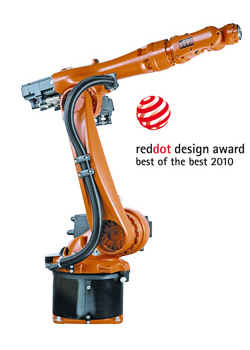
\includegraphics[width=0.58\textwidth]{PR_KR5_arc_02}
\caption{Robot KUKA KR5 Arc. Převzato z \cite{kuka_datasheet_url}.}
\label{kuka_kr5_pic}
\end{figure}

Tento robot s hmotností 127 kg a základní nosností 5 kg patří mezi lehčí průmyslové roboty. Byl vyvinut primárně pro aplikace vyžadující vysokou přesnost polohování, jako je obloukové svařování a přesná manipulace s lehkými pevnými předměty. Robot je schopen polohovat koncový efektor s přesností do 0,04 mm. Objem pracovní obálky je 8,4 \si{m^{3}}. Díky lehké konstrukci a výkonným pohonům o je robot schopen dosahovat vysokých provozních rychlostí s rychlostí koncového efektoru přesahující 5 \si{m/s}.  

\begin{figure}[ht]
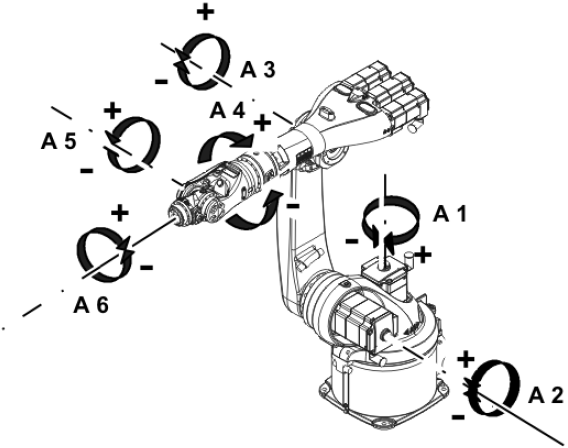
\includegraphics[width=0.8\textwidth]{kuka_kr5_axes}
\caption{Konfigurace os robota. Převzato z \cite{kuka_datasheet_url}.}
\label{kuka_kr5_axes_pic}
\end{figure}

Jako pohony os jsou použity třífázové synchronní servopohony s permanentními magnety (PMSM). Pro zvýšení točivého momentu motorů a přesnosti polohování jsou motory opatřeny převodovkou. Servomotory robota jsou vybaveny snímači pro snímání úhlu natočení rotoru, sondami pro měření proudu protékajícího jejich vinutím a tepelnými senzory pro měření teploty uvnitř motoru. Jednotlivé osy jsou dále vybaveny brzdným mechanismem, který zabraňuje otáčení os, pokud není robot v aktivním pohybu. 

Součástí robota je i řídicí systém zajišťující napájení a řízení robota a poskytující uživatelské rozhraní (HMI) pro jeho programování a ovládání. Pohyb robota je programován v jazyce KRL (KUKA Robot Language). Součástí řídicího systému je i užitečný nástroj TRACE, umožňující sledování vnitřních stavů robota jako jsou polohy, rychlosti a zrychlení jednotlivých os, jejich momenty, protékající proudy a mnoho dalších. 

Celý systém je napájen z třífázové soustavy elektrické energie. Je určen pro montáž na zem nebo strop ve vnitřních prostorách. Podrobnější informace je možné nalézt v katalogovém listu. \cite{kuka_datasheet_url}.